%-----------------------------------------------------------------------------
%
%               Template for sigplanconf LaTeX Class
%
% Name:         sigplanconf-template.tex
%
% Purpose:      A template for sigplanconf.cls, which is a LaTeX 2e class
%               file for SIGPLAN conference proceedings.
%
% Guide:        Refer to "Author's Guide to the ACM SIGPLAN Class,"
%               sigplanconf-guide.pdf
%
% Author:       Paul C. Anagnostopoulos
%               Windfall Software
%               978 371-2316
%               paul@windfall.com
%
% Created:      15 February 2005
%
%-----------------------------------------------------------------------------


%\documentclass[preprint]{sigplanconf}
\documentclass[10pt]{sigplanconf}

% The following \documentclass options may be useful:
%
% 10pt          To set in 10-point type instead of 9-point.
% 11pt          To set in 11-point type instead of 9-point.
% authoryear    To obtain author/year citation style instead of numeric.

\usepackage{yfonts}
\usepackage{amsmath}
\usepackage{amsthm}
\usepackage{amssymb}
%\usepackage{mathpartir}
\usepackage{hyperref}
\usepackage{url}
\usepackage{graphics}
\usepackage{graphicx}
\usepackage{wasysym}
\usepackage{harmony}
\usepackage{marvosym}
\usepackage{multirow}
\usepackage[usenames,dvipsnames]{xcolor}
\usepackage[utopia]{mathdesign}
\usepackage{natbib}
\usepackage[mathcal]{euscript}
\usepackage[linesnumbered,ruled]{algorithm2e}

\renewcommand{\UrlBreaks}{\do\/\do\a\do\b\do\c\do\d\do\e\do\f\do\g\do\h\do\i\do\j\do\k\do\l\do\m\do\n\do\o\do\p\do\q\do\r\do\s\do\t\do\u\do\v\do\w\do\x\do\y\do\z}

% ____________________________________________________________
% Listings Package Configuration
% \usepackage[scaled]{beramono}

%\renewcommand*\ttdefault{txtt}
\usepackage[T1]{fontenc}

% This Deep Tex Voodoo is from
%   <http://www.latex-community.org/forum/viewtopic.php?f=5&t=2072>
% It's purpose is to make \lstinline normal size, without affecting
% \lstinputlisting.  It seems to work but I have no idea how or why,
% and I rather hope never to learn.
%\makeatletter
%\lst@AddToHook{TextStyle}{\let\lst@basicstyle\ttfamily\normalsize}
%\makeatother

\begin{document}

\conferenceinfo{SIGBOVIK '17}{Pittsburgh, PA, USA}
\copyrightyear{2017}
\copyrightdata{}

\titlebanner{banner above paper title}        % These are ignored unless
\preprintfooter{short description of paper}   % 'preprint' option specified.

\title{
A Boring Follow-Up Paper to \\
``Which ITG Stepcharts are Turniest?'' \\
Titled, ``Which ITG Stepcharts are Crossoveriest and/or Footswitchiest?'' \\
%That `Boring' Stuff Was Part of the Title, BTW. \\
%So was that. And that, and this too. \\
%You got it all, right? \\
%Or Just, ``More Boring Crap about ITG'', for Short. \\
%Oh, That Was Also Part of the Title.
}
% \subtitle{\em The Randomly-Scoped Lambda Calculus}
% \subtitle{Subtitle Text, if any}

\authorinfo{Ben Blum}{}{bblum@cs.cmu.edu}

\maketitle

\begin{abstract}
	%ITG is a popular dance game in which players step on arrows while listening to music. The arrow patterns, indicated by a {\em stepchart}, may range among any level of complexity and difficulty. Among the many factors contributing to a stepchart's difficulty is how much the player must turn from side to side.
	%Other more obvious factors, such as raw speed, have been well studied in prior work.
	%This paper presents an analytic study of this {\em turniness} factor.
	%We study the turniness of many existing stepcharts, and present a novel (but unsurprising) approach to automatically generating maximally (or minimally) turny charts.
	%Among real-world songs, we find stepcharts with overall turniness ranging from 0\% to 81.33\% of the theoretical maximum.

In which I deliver on last year's promise of future work.

\end{abstract}

\category{D.D.R.}{Exercise and Fitness}{Arcade Dance Games}

\keywords
crossovers, footswitches, jacks, sidefoots


\section{Introduction}

Let's resume right where I left off in my last paper \cite{turniness}, shown in Figure~\ref{fig:you-stutid-fuckass}.
Unlike mainstream conferences, SIGBOVIK doesn't make me waste space repeating all the background material,
and I can just say go read that paper first and get back to me.
It's probably a lot funnier than this one anyway, which is gonna be sort of dry,
and really of interest only to other ITG players who already know what's going on.

\begin{figure}[h]
	\hspace{-2em}\includegraphics[angle=90,width=0.54\textwidth]{../paper.pdf}
	\caption{(okay twist your head to read this)}
	\label{fig:you-stutid-fuckass}
\end{figure}

The TL;DR is that I made a program which figures out how to foot stepcharts in the least crossovery possible way (short of double-stepping everything),
then found which charts ultimately had the most.
The algorithm also naturally identifies footswitches and jacks, %, jacks, forced double-steps, and crossover-footswitches;
and sometimes it's smarter than me in amusing ways.
I put all the goodies in a giant spreadsheet at \url{http://tinyurl.com/crossoveriest},
and the program itself is of course freely available at \url{https://github.com/bblum/sigbovik/blob/master/itg/code/ITG.hs}.



%%%%%%%%%%%%%%%%%%%%%%%%%%%%%%%%%%%%%%%%%%%%%%%%%%%%%%%%%%%%%%%%%%%%%%%%%%%%%%%%

\section{Revisiting Turniness (Flashback Scene)}

Recall Table~\ref{tab:facing} from the last paper, in which I left undefined the facings for $LL$, $DD$, $UU$, and $RR$, the four footswitches.
I show a typical $DD$/$UU$ footswitch pattern in Figure~\ref{fig:fs}(a), and typical $LL$/$RR$ switches (henceforth ``crossover footswitches'') in Figure~\ref{fig:fs}(b).
To step these patterns, the player still alternates feet as usual, but must lift one foot off the repeated arrow before stepping it with her other foot.
Chart authors will often, but not always, include a ``mine cue'' (shown in the figure) to hint that the second foot should switch onto the same arrow.

\begin{table}[t]
	\begin{center}
	\begin{tabular}{cc|cccc}
		& & \multicolumn{4}{c}{Right foot} \\
		& & $\leftarrow$ & $\downarrow$ & $\uparrow$ & $\rightarrow$ \\
		\hline
		\multirow{4}{*}{Left foot}
		%                 L   D   U   R
		& $\leftarrow$  & \bf ? & $UR$ & $UL$ & $U$ \\
		& $\downarrow$  & $DL$ & \bf ? & $L$ & $UL$ \\
		& $\uparrow$    & $DR$ & $R$ & \bf ? & $UR$ \\
		& $\rightarrow$ & $D$ & $DR$ & $DL$ & \bf ? \\

	\end{tabular}
	\end{center}
	\caption{Facing directions.
	%``Crossover'' facings are marked (*), and the ``lateral'' facing is marked ($\dagger$). Note the appealing diagonal symmetry.}
	}
	\label{tab:facing}
\end{table}

\begin{figure}[t]
	\begin{tabular}{c}
	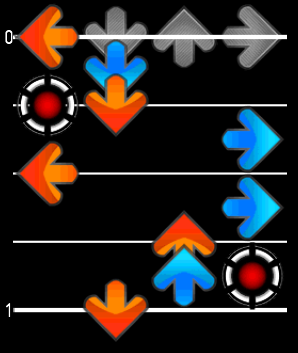
\includegraphics[width=0.13\textwidth]{fs-dd-uu.png} \\
	(a) DD, UU
	\end{tabular}
	\begin{tabular}{c}
	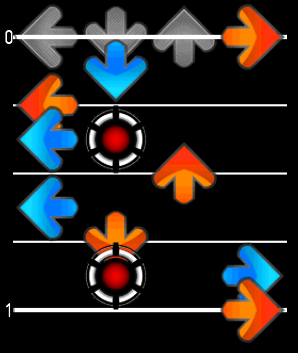
\includegraphics[width=0.13\textwidth]{fs-ll-rr.png} \\
	(b) LL, RR
	\end{tabular}
	\begin{tabular}{c}
	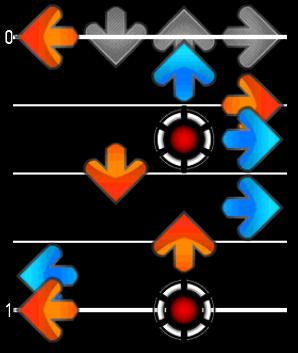
\includegraphics[width=0.13\textwidth]{fs-ll-rr-2.png} \\
	(c) RR, LL
	\end{tabular}
	\caption{Footswitches of various crossoveriness/facing.}
	\label{fig:fs}
\end{figure}

It is tempting to assign the facings $L$, $U$, $U$, and $R$ respectively to the $LL$, $DD$, $UU$, and $RR$ footswitches.
However, Figure~\ref{fig:fs}(c) shows that if a footswitch begins with a crossover on $U$, the facing should be reversed:
the $RR$ footing should face $L$, and $LL$ should face $R$.
``Spin-switches'' with $D$ facing are also theoretically possible,
arising from patterns such as $LURDDL$ or $LDRUUL$,
%although I know of no real-world chart which does this (hmm, tempting...).
or similarly, ``270-switches'', as shown in Figure~\ref{fig:real-world-turniness}(a).

Before I realized that, I modified the turniness algorithm \cite{turniness} to face footswitches as above, %the bad way mentioned above,
%to be faced $L$ for $LL$ and so on, as above,
and it surprised me with charts of $\mathcal{T}>2$, in excess of the theoretical maximum!
I show one such chart in Figure~\ref{fig:fs-turniness}(a), in which the step from $LL$ ($\phi=L$) to $UL$ ($\phi=DR$) has individual $\mathcal{T}=3$, and so on for $UL \rightsquigarrow_R UU \rightsquigarrow_L RU \rightsquigarrow_R RR$.
The steps $RR \rightsquigarrow_L LR \rightsquigarrow_R LL$ are both candles ($\mathcal{T}=2$),
resulting overall in $\mathcal{T}=8/3$ for the whole chart.

Indeed, when I further modified the algorithm to force $DD$ switches to face $D$ (i.e., always facing the direction of the repeated arrow),
it produced the chart shown in Figure~\ref{fig:fs-turniness}(b), with overall $\mathcal{T}=3$.
(Note its resemblance to the basic spin pattern, $LDRU$, whose $\mathcal{T}=2$.)

To fairly represent a human player's desire to step in the least turny of ambiguous ways,
I extended the algorithm to provide either the assigned facing, from above, or its polar opposite,
chosen at runtime by whichever is closer to the presequent facing.
This restores the maximum overall chart turniness to $\mathcal{T}=2$,
a new example of which is shown in Figure~\ref{fig:fs-turniness}(c).
Figure~\ref{fig:real-world-turniness}(b) also shows a real-world chart exhibiting this pattern.

However, note that individual steps may still have $\mathcal{T}=3$,
%because after a footswitch's facing is determined, the next step may still ... ?
as shown in Figure~\ref{fig:fs-turniness}(d).
In this example, the step $DL \rightsquigarrow_L LL$ assigns $LL$ to face $L$,
but the subsequent step to $LD$ cannot avoid facing $UR$.
The reason charts still cannot exceed overall $\mathcal{T}=2$ is that
setting up such a situation requires a $\mathcal{T}=1$ step,
which negates the benefit.
A chart could conceivably end right before such a step,
sneaking through some small $\epsilon$ extra turniness \cite{epsilon}
(similar to the case of 270s in \cite{turniness}),
but {\em sustained} average $\mathcal{T}>2$ remains impossible.

Another approach could assign such a footswitch the opposite footing of the previous facing,
regardless of the arrow itself;
so in this case the $LL$ would face $UL$, and each step would have exactly $\mathcal{T}=2$.
%Anyway, remember that all-candle switch stream in (c). We'll see it again soon.

\begin{figure}[t]
	\begin{center}
	\begin{tabular}{c}
	\begin{tabular}{c}
	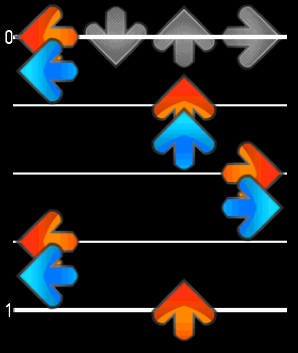
\includegraphics[width=0.13\textwidth]{fs-turniness-8-3.png} \\
	(a) $\mathcal{T}=8/3$(?)%\stackrel{?}{=}8/3$
	\end{tabular}
	\begin{tabular}{c}
	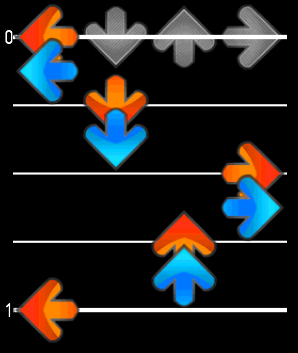
\includegraphics[width=0.13\textwidth]{fs-turniness-3.png} \\
	(b) $\mathcal{T}=3$(?)%\stackrel{?}{=}3$
	\end{tabular}
	\\
	\\
	\begin{tabular}{c}
	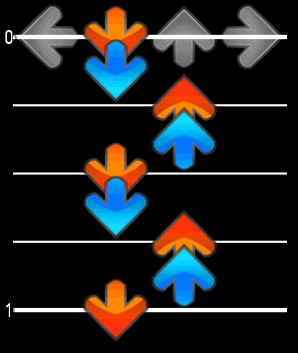
\includegraphics[width=0.13\textwidth]{fs-turniness-2.png} \\
	(c) $\mathcal{T}=2$.
	\end{tabular}
	\begin{tabular}{c}
	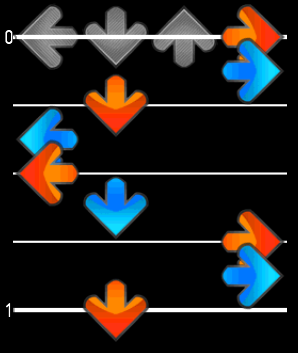
\includegraphics[width=0.13\textwidth]{fs-turniness-2-plus-epsilon.png} \\
	(d) $\mathcal{T}=2+\epsilon$.
	\end{tabular}
	\end{tabular}
	\end{center}
	\caption{The turniest footswitch patterns. (a) and (b) are false positives (see prose), while (c) and (d) provide theoretically maximal turniness.}
	\label{fig:fs-turniness}
\end{figure}

\begin{figure}[t]
	\begin{center}
	\begin{tabular}{c}
		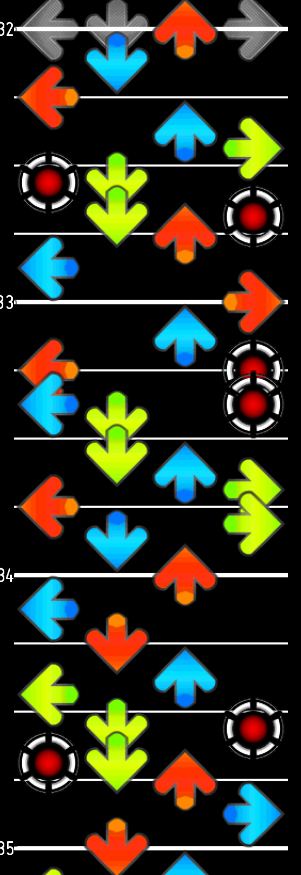
\includegraphics[width=0.16\textwidth]{web33-dd-switch-270.png}
		\\
		(a) Web33,260.8 \\
		(12, Rikame 5)
	\end{tabular}
	\begin{tabular}{c}
		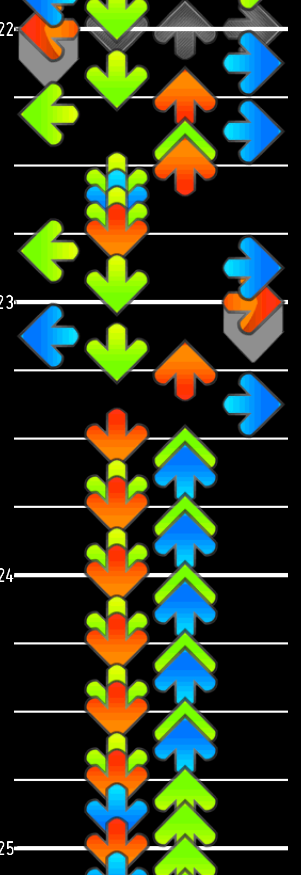
\includegraphics[width=0.16\textwidth]{fuego-candle-fs.png}
		\\
		(b) Fuego \\
		(12, Best of Gazebo)
	\end{tabular}
	\end{center}
	\caption{Real-world examples of turny footswitches.}
	\label{fig:real-world-turniness}
\end{figure}


% dont forget
% http://dancedancerevolutionddr.wikia.com/wiki/Afronova_walk

%%%%%%%%%%%%%%%%%%%%%%%%%%%%%%%%%%%%%%%%%%%%%%%%%%%%%%%%%%%%%%%%%%%%%%%%%%%%%%%%

\section{Analyzing Crossoveriness}

\newcommand\hilight[2]{\color{#1}#2\color{black}}
\definecolor{pink}{RGB}{128,0,192}
\definecolor{orange}{RGB}{192,96,0}
\definecolor{olivegreen}{RGB}{0,127,32}
\definecolor{brickred}{RGB}{192,0,0}
\definecolor{commentblue}{RGB}{0,128,192}

\begin{figure*}[ht]
\begin{tabular}{l}
\texttt{\hilight{orange}{data}~\hilight{olivegreen}{Step}~= \hilight{brickred}{L}~| \hilight{brickred}{D}~| \hilight{brickred}{U}~| \hilight{brickred}{R}~| \hilight{brickred}{Jump}~\hilight{orange}{deriving}~\hilight{olivegreen}{Eq}} \\
\texttt{} \\
\texttt{\hilight{orange}{data}~\hilight{olivegreen}{AnalysisState}~= \hilight{brickred}{S}~\{ steps :: \hilight{olivegreen}{Int}, xovers :: \hilight{olivegreen}{Int}, switches :: \hilight{olivegreen}{Int}, jacks :: \hilight{olivegreen}{Int},} \\
\texttt{~~~~~~~~~~~~~~~~~~~~~~~~ lastStep :: \hilight{olivegreen}{Maybe}~\hilight{olivegreen}{Step}, doubleStep :: \hilight{olivegreen}{Bool}, lastFlip :: \hilight{olivegreen}{Bool},} \\
\texttt{~~~~~~~~~~~~~~~~~~~~~~~~ lastFoot :: \hilight{olivegreen}{Bool}, stepsLR :: [\hilight{olivegreen}{Bool}] \}} \\
\texttt{} \\
\texttt{\hilight{pink}{commitStream}~:: \hilight{olivegreen}{AnalysisState}~-> \hilight{olivegreen}{AnalysisState}} \\
\texttt{\hilight{pink}{commitStream}~s = s \{ xovers~~ = xovers~~ s + \hilight{orange}{if}~f \hilight{orange}{then}~ns - nx \hilight{orange}{else}~nx, } \\
\texttt{~~~~~~~~~~~~~~~~~~~~ switches = switches s + \hilight{orange}{fromEnum}~(f == lastFlip s \&\& doubleStep s), } \\
\texttt{~~~~~~~~~~~~~~~~~~~~ jacks~~~~= jacks~~~~s + \hilight{orange}{fromEnum}~(f /= lastFlip s \&\& doubleStep s), } \\
\texttt{~~~~~~~~~~~~~~~~~~~~ lastFlip = f, stepsLR = \hilight{brickred}{[]}~\}} \\
\texttt{~~~~\hilight{orange}{where}~ns = \hilight{orange}{length}~\$~stepsLR s} \\
\texttt{~~~~~~~~~~nx = \hilight{orange}{length}~\$ \hilight{orange}{filter not}~\$ stepsLR s} \\
%\texttt{~~~~~~~~~~\hilight{commentblue}{-{}- if more than half the L/R steps in this stream were crossed over,}} \\
%\texttt{~~~~~~~~~~\hilight{commentblue}{-{}- then we got the footing backwards and need to flip the stream.}} \\
%\texttt{~~~~~~~~~~\hilight{commentblue}{-{}- as a tiebreaker, flip if the chart is already more jacky than}} \\
%\texttt{~~~~~~~~~~\hilight{commentblue}{-{}- footswitchy, i.e., if past streams flipped more often than not.}} \\
\texttt{~~~~~~~~~~\hilight{commentblue}{-{}- reverse the stream's footing if more L/R steps were crossed over than not.}} \\
\texttt{~~~~~~~~~~f = nx * 2 > ns || nx * 2 == ns \&\& ((switches s > jacks s) == lastFlip s)} \\
\texttt{} \\
\texttt{\hilight{pink}{analyzeStep}~:: \hilight{olivegreen}{AnalysisState}~-> \hilight{olivegreen}{Step}~-> \hilight{olivegreen}{AnalysisState}} \\
\texttt{\hilight{pink}{analyzeStep}~s step} \\
%\texttt{~~~~\hilight{commentblue}{-{}- a jump resets the footing, so the next step can be stepped with either}} \\
%\texttt{~~~~\hilight{commentblue}{-{}- foot. commit the stream so far to treat it separately from what follows.}} \\
%\texttt{~~~~\hilight{commentblue}{-{}- bracket-jumps are, of course, future work.}} \\
\texttt{~~~~| step == \hilight{brickred}{Jump}~= (\hilight{pink}{commitStream}~s) \{ lastStep = \hilight{brickred}{Nothing}, doubleStep = \hilight{brickred}{False}~\}} \\
%\texttt{~~~~\hilight{commentblue}{-{}- two steps on the same arrow might be a jack, or might be a footswitch.}} \\
%\texttt{~~~~\hilight{commentblue}{-{}- to figure out which, commit the stream so far, and begin a new stream}} \\
%\texttt{~~~~\hilight{commentblue}{-{}- whose footing will retroactively determine how to foot this step.}} \\
%\texttt{~~~~\hilight{commentblue}{-{}- also, unlike jumps, this step gets counted as part of the next stream.}} \\
\texttt{~~~~| lastStep s == \hilight{brickred}{Just}~step = stream (\hilight{pink}{commitStream}~s) \{ doubleStep = \hilight{brickred}{True}~\}} \\
%\texttt{~~~~\hilight{commentblue}{-{}- a normal streamy step.}} \\
\texttt{~~~~| \hilight{orange}{otherwise}~= stream s} \\
\texttt{~~~~\hilight{orange}{where}~foot = \hilight{orange}{not}~\$ lastFoot s} \\
\texttt{~~~~~~~~~~\hilight{commentblue}{-{}- record whether we stepped on a matching or crossed-over L/R arrow.}} \\
\texttt{~~~~~~~~~~addStep ft \hilight{brickred}{L}~steps = steps ++ [ft]} \\
\texttt{~~~~~~~~~~addStep ft \hilight{brickred}{R}~steps = steps ++ [\hilight{orange}{not}~ft]} \\
\texttt{~~~~~~~~~~addStep ft \_ steps = steps \hilight{commentblue}{-{}- U/D don't help to determine L/R footing.}} \\
\texttt{~~~~~~~~~~stream s = s \{ steps = steps s + \hilight{brickred}{1}, lastStep = \hilight{brickred}{Just}~step, lastFoot = foot,} \\
\texttt{~~~~~~~~~~~~~~~~~~~~~~~~ stepsLR = addStep foot step \$ stepsLR s \} } \\
\texttt{} \\
\texttt{\hilight{pink}{analyze}~:: [\hilight{olivegreen}{Step}] -> \hilight{olivegreen}{AnalysisState}} \\
\texttt{\hilight{pink}{analyze}~= \hilight{pink}{commitStream}~. \hilight{orange}{foldl}~\hilight{pink}{analyzeStep}~(\hilight{brickred}{S 0 0 0 0}~\hilight{brickred}{Nothing}~\hilight{brickred}{False}~\hilight{brickred}{False}~\hilight{brickred}{False}~\hilight{brickred}{[]}) } \\
\end{tabular}
	\caption{Pseudocode description of the crossoveriness and footswitchiness algorithm.}
\label{fig:pseudocode}
\end{figure*}

The major flaw of the turniness algorithm \cite{turniness}
was that it didn't care whether a stream started with the left or right foot;
it simply exploited the symmetry of Table~\ref{tab:facing} to find turniness regardless of footing.
Hence, it could not distinguish technical footing patterns which could affect the way a human would play the chart.
It often played charts inhumanly, facing backwards and/or stepping 270s for most of a song.

So, my contribution this year is an algorithm which plays more naturally,
and which consequently can report on a chart's technical patterns beyond simple turniness.
The algorithm realizes three principles of ITG:
\begin{enumerate}
	\item Alternate feet as much as possible.
	\item Step crossed-over as little as possible.
	\item Jumps or jacks allow the player to reset her footing.
\end{enumerate}

Figure~\ref{fig:pseudocode} describes the algorithm in pseudocode.
To summarize it in prose:
\begin{itemize}
	\item Split the chart into several units of stream,
		the boundaries of which occur at every jump and any time an arrow is repeated.
	\item Step each stream with alternating feet.
	\item Compare the number of matching steps (i.e., $L$ foot on $L$ arrow or $R$ on $R$) versus crossover steps.
		If the latter is greater, re-step the stream with opposite feet from before (this kills the crossovers).
	\item After flipping each stream, if necessary, count the total crossovers in the whole chart.
\end{itemize}

\section{Analyzing Footswitchiness}

Because we split the chart whenever an arrow is repeated,
figuring out whether that arrow is stepped with different feet on either side of the stream boundary
is a natural consequence of figuring out how to step each stream individually.
This is also shown in Figure~\ref{fig:pseudocode}'s pseudocode.
To summarize in prose,
if neither stream needed to be flipped (or if both did), then the alternating feet assumption holds,
and the repeat must be a footswitch.

\section{Analyzing Jackiness}

A jack occurs when a repeat arrow is stepped with the same foot,
rather than alternating (hence the name, from ``jackhammer'').
You've got the idea by now, right?


%%%%%%%%%%%%%%%%%%%%%%%%%%%%%%%%%%%%%%%%%%%%%%%%%%%%%%%%%%%%%%%%%%%%%%%%%%%%%%%%

\section{Forced Doublesteps}

After painstakingly translating the pseudocode from Figure~\ref{fig:pseudocode} into a real implementation,
I found it vulnerable to false positives when a single double-step could force a long section of stream to be stepped backwards.
As an extreme example, consider the pattern $LRLRLRLR-D-LRLRLRLR$.
Because no jumps or jacks allow the footing to be reset, either the first or last 4 pairs of $LR$s must be stepped crossed-over.

Figure~\ref{fig:force-doublestep} shows two examples from real-world charts:
in (a), the player must not alternate feet across the measure break,
while in (b), two $L$ arrows are replaced with rolls for an artistic visual accent, which must be stepped twice each.
On inspection, these charts should be stepped with no crossovers, but were evaluated otherwise %as having very high XO\%
%(anywhere from 10.6\% to 27.9\%).
(730 XOs (27.9\%) and 173 XOs (9.6\%), respectively).

\begin{figure}[t]
	\begin{center}
	\begin{tabular}{c}
		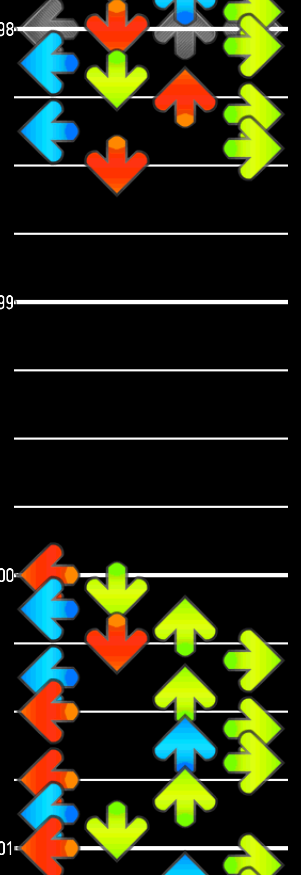
\includegraphics[width=0.16\textwidth]{paradise-lost-false-positive.png}
		\\
		(a) Paradise Lost \\
		(16, Cirque du Lykan)
	\end{tabular}
	\begin{tabular}{c}
		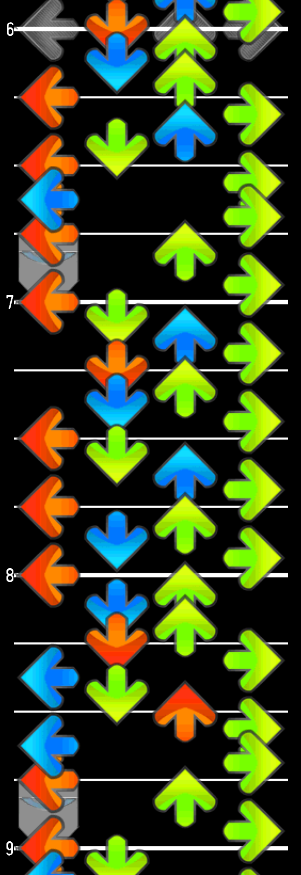
\includegraphics[width=0.16\textwidth]{hearbeat-rollstream-doublestep.png}
		\\
		(b) Heartbeat \\
		(13, TranceNation)
	\end{tabular}
	\end{center}
	\caption{The doublesteps in some streamy charts must be identified, and the stream split, lest ``too much'' of the following stream appear completely crossed-over.}
	\label{fig:force-doublestep}
\end{figure}

\newcommand\Stream{\ensuremath{\mathcal{S}}}
\newcommand\Doublestep{\ensuremath{\mathcal{DS}}}
\newcommand\nflip{\ensuremath{n_{\mathfrak{flip}}}}
\newcommand\percentflip{\ensuremath{\%_{\mathfrak{flip}}}}
\begin{algorithm}[h]
	\SetKwInOut{Input}{Input}
	\SetKwInOut{Output}{Invariant}
	\Input{\Stream, a step sequence $s_0 \dots s_n$}
	\Output{$\forall s_i, s_j \in \Stream, j=i+1 \rightarrow \mathsf{\neg StreamBoundary}(s_i,s_j)$}
	\Input{\nflip, heuristic minimum length} %of flipped stream to doublestep into}
	\Input{$\percentflip$, heuristic percentage, initially 100}
	\For{$i \in \mathsf{length}(\Stream) \wedge \neg {\sf defined}(i_{\Doublestep})$}{
		$\Stream' \leftarrow \{ s_k | s_k \in \mathsf{LRs}(\{ s_j | s_j \in \Stream \wedge j \ge i \}) \wedge k \le \nflip \}$ \\
		\If{$|\Stream'| = \nflip$ $\wedge$ $|\mathsf{Crossovers}(\Stream')| \ge \percentflip \times |\Stream'|$}{
			$i_{\Doublestep} \leftarrow i$
		}
	}
	\eIf{{\sf defined}($i_{\Doublestep})$}{
		\If{$i_{\Doublestep} = 0$}{
			% gotta write "tail stream" as complicatedly as possible
			$i_{\Doublestep} \leftarrow \mathsf{FindUnflippedSection}(\{ s_i | s_i \in \Stream \wedge i \ne 0 \})$
			%\mathsf{tail}(\Stream))$
		}
		{\sf HeuristicallyDoublestep}($\{ s_i | s_i \in \Stream \wedge i < i_{\Doublestep} \}$)
		{\sf HeuristicallyDoublestep}($\{ s_i | s_i \in \Stream \wedge i \ge i_{\Doublestep} \}$)
	}{
		{\sf CommitStream}(\Stream)
	}
	\caption{{\sf HeuristicallyDoublestep}(\Stream)}
	\label{alg:heuristic}
\end{algorithm}

To handle such cases,
I extended the algorithm with a heuristic to identify when a stream becomes ``too crossed-over'' for ``too long'',
and to force a doublestep by splitting the stream to flip it back.
Algorithm~\ref{alg:heuristic} shows the implementation.
I will not summarize how it works due to space limitations, but the description should be intuitive enough.
The heuristic evaluated Figure~\ref{fig:force-doublestep}'s charts as having 0 crossovers each and 1 and 21 doublesteps, respectively.
In my analysis next section, I will use $\nflip = 9$
(determined by inspection of a few favourite charts, which should be scientifically rigorous enough for anyone).

%%%%%%%%%%%%%%%%%%%%%%%%%%%%%%%%%%%%%%%%%%%%%%%%%%%%%%%%%%%%%%%%%%%%%%%%%%%%%%%%

\section{Evaluation}

Our experimental corpus has grown considerably since last year, and now comprises 11,666 stepcharts.
I ran the crossoveriness/etcetera algorithm on all of them,
and counted the total steps (not including jumps), crossovers, footswitches, jacks, forced doublesteps, and crossover switches for each.
I also grouped the charts by author and by song pack to calculate each author's/pack's overall crossoveriness/etc.
You can view the entire dataset at \url{http://tinyurl.com/crossoveriest}.

Tables
\ref{tab:chart-xo},
\ref{tab:chart-xop},
\ref{tab:chart-fs},
\ref{tab:chart-fsp},
\ref{tab:chart-xf},
\ref{tab:author-xo},
\ref{tab:author-fs},
\ref{tab:author-jk},
\ref{tab:pack-xo},
\ref{tab:pack-fs},
and
\ref{tab:pack-jk}
summarize the dataset as ``leaderboards'' for each category.
They present the data the same way as last year \cite{turniness},
so I won't explain it again.
Suffice to say that ITG enthusiasts should use their personal chart style preferences to navigate these tables and find song or pack recommendations or feel proud of themselves or whatever.

In the by-author analysis, I excluded authors with fewer than 10 charts, like last time.
Also, in by-author and by-pack, I excluded 1-, 2-, and 3-foot charts,
on the pretense that they often ignore the alternating feet assumption
(though I also admit this biases the analysis against DDR/Konami).
%(though I also admit some bias in wanting to unseat DDR/Konami as the crossover king).
Nevertheless, DDR charts generally ruled the single-digits,
even in footswitchiness,
showing perhaps more technical depth than I gave them credit for.
%Also, congratulations to Fraxtil and S. Tofu, who managed to write not a single crossover or footswitch, respectively.

By the way, the theoretical maxima for XO\%, FS\%, and JK\% are 50-$\epsilon$, 100-$\epsilon$, and 100-$\epsilon$, respectively \cite{epsilon}.

% charts
\begin{table}[t]
	\begin{center}
		\small
	\begin{tabular}{r|l|l|l}
		\bf Ft. & \bf Name & \bf Pack & \bf \#XO \\
		\hline
		 6 & Autoload                 & ITG 3                 &  54 \\
		 7 & Tetris                   & CuoReNeRo M'PacK      &  58 \\
		 8 & Pulse                    & CuoReNeRo M'PacK      &  94 \\
		 9 & MAX Forever              & CuoReNeRo M'PacK      & 107 \\
		10 & J-PARA SUPER MEGAMIX     & CuoReNeRo M'PacK      & 141 \\
		11 & Somebody I Used To Know  & Best of Gazebo        & 114 \\
		12 & Credens Justitiam        & Stuff B Likes         & 136 \\
		13 & Banshee Strikes          & VocaJawnz             & 152 \\
		14 & Slow Down                & Sexuality Violation 2 & 160 \\
		15 & yoshikawa45 vs siesta45  & Rikame's Simfiles 4   & 111 \\
		16 & Your Best Nightmare      & Undertale             &  97 \\
		\multicolumn{4}{c}{\em no 17s-19s with $\ge$50 XOs} \\
		20 & Rainbow Dimension        & Rikame's Simfiles 2   &  84 \\
		21 & Teenage Dream            & Sexuality Violation 2 & 280 \\
	\end{tabular}
	\end{center}
	\caption{Charts with the most total crossovers (XOs).}
	\label{tab:chart-xo}
\end{table}
\begin{table}[t]
	\begin{center}
		\small
	\begin{tabular}{r|l|l|l}
		\bf Ft. & \bf Name & \bf Pack & \bf XO\% \\
		\hline
		 4 & DAM DIRIRAM              & DDR 3rdMIX            & 27.3 \\
		 5 & STRICTLY BUSINESS        & DDR 1st               & 21.4 \\
		 6 & STRICTLY BUSINESS        & DDR 1st               & 20.9 \\
		 7 & MOBO$\star$MOGA          & DDR EXTREME           & 17.3 \\
		 8 & PARANOiA                 & DDR 1st               & 19.6 \\
		 9 & Dazzlin Darlin           & r21twins              & 22.0 \\
		10 & Enchanted Journey        & ITG Rebirth           & 19.3 \\
		11 & Lune Noir                & r21freak Friendship   & 13.4 \\
		12 & W'peg is Fucking Over    & best of r21freak ii   & 14.3 \\
		13 & The Sampling Paradise    & The Paradise Sampler  & 15.6 \\
		14 & Slow Down                & Sexuality Violation 2 & 13.3 \\
		15 & yoshikawa45 vs siesta45  & Rikame's Simfiles 4   & 10.8 \\
		\multicolumn{4}{c}{\em no 16s-19s with $\ge$10\% XO} \\
		20 & Rainbow Dimension        & Rikame's Simfiles 2   & 10.7 \\
		21 & Teenage Dream            & Sexuality Violation 2 & 11.8 \\
	\end{tabular}
	\end{center}
	\caption{Charts with the highest percentage of XOs among total steps.}
	\label{tab:chart-xop}
\end{table}
\begin{table}[t]
	\begin{center}
		\small
	\begin{tabular}{r|l|l|l}
		\bf Ft. & \bf Name & \bf Pack & \bf \#FS \\
		\hline
		%\multicolumn{4}{c}{\em no 5s- with $\ge$50 FSs} \\
		 6 & Sweat Shop       & ITG Rebirth 2 Beta    &  56 \\
		 7 & Silent Hill      & DDR 3rdMIX            &  29 \\
		 8 & Pulse            & CuoReNeRo M'PacK      &  41 \\
		 9 & Dr. Boom-Bombay  & fort rapids vii       &  34 \\
		10 & Eat 'Em Up!      & Mute Sims 5           &  54 \\
		11 & Nemeton          & The Legend of Zim 4   &  97 \\
		12 & Nemeton          & Subluminal            & 140 \\
		13 & Love Is Eternity & Subluminal            & 140 \\
		14 & Switch           & Getty                 & 347 \\
		15 & Danse Macabre    & Aoreo's Ariginals     & 201 \\
		16 & Weird Science    & Stamina Showcase      &  61 \\
		17 & Arcane Apparatus & Tachyon Gamma         &  32 \\
		18 & Metallic-A-      & Oh Henry! Mad Stamina &  27 \\
		19 & Geronimo         & Sexuality Violation 3 &  39 \\
		20 & Scatman's World  & Jimmy Jawns 2         &  22 \\
		21 & He He He         & Jimmy Jawns 2         &   4 \\
		22 & Architecture     & SPEEEDCOOOORE 4       &  24 \\
		23 & Geronimo         & Sexuality Violation 3 &  39 \\
	\end{tabular}
	\end{center}
	\caption{Charts with the most total footswitches (FSs).}
	\label{tab:chart-fs}
\end{table}
\begin{table}[t]
	\begin{center}
		\small
	\begin{tabular}{r|l|l|l}
		\bf Ft. & \bf Name & \bf Pack & \bf FS\% \\
		\hline
		 3 & Sweat Shop       & ITG Rebirth 2 Beta    & 15.3 \\
		 4 & DROP THE BOMB    & DDR 3rdMIX            &  9.8 \\
		 5 & MAKE IT BETTER   & DDR 2ndMIX            & 20.0 \\
		 6 & Sweat Shop       & ITG Rebirth 2 Beta    & 18.2 \\
		 7 & 5.1.1            & DDR MAX               & 12.9 \\
		 8 & La Se\~{n}orita Virtual & DDR 3rdMIX     &  8.4 \\
		 9 & PARANOiA KCET    & DDR 2ndMIX            & 10.2 \\
		10 & Delhi Ill        & Mute Sims 6           & 11.6 \\
		11 & Sweat Shop       & ITG Rebirth 2 Beta    & 11.8 \\
		12 & Nemeton          & Subluminal            & 14.8 \\
		13 & Love Is Eternity & Subluminal            & 16.8 \\
		14 & Switch           & Getty                 & 15.7 \\
		15 & Flames of the Sky & fort rapids vii      & 16.5 \\
		16 & Mermaid Island   & Tachyon Alpha         &  9.5 \\
		\multicolumn{4}{c}{\em no 17s+ with $\ge$5\% FS} \\
	\end{tabular}
	\end{center}
	\caption{Charts with the highest percentage of FSs.} %among total steps.}
	\label{tab:chart-fsp}
\end{table}
\begin{table}[h!]
	\begin{center}
		\small
	\begin{tabular}{r|l|l|l}
		\bf Ft. & \bf Name & \bf Pack & \bf \#XF \\
		\hline
		\multicolumn{4}{c}{\em no 8s- with $\ge$12 XFs} \\
		 9 & Dr. Boom-Bombay   & fort rapids vii            & 18 \\
		10 & Toxic             & Sexuality Violation 2      & 12 \\
		11 & Heart Shooter     & VocaJawnz                  & 44 \\
		12 & Web 33,260.8      & Rikame's Simfiles 5        & 16 \\
		13 & Toxic             & Sexuality Violation 2      & 12 \\
		14 & Fancy Footwork    & Cirque du Zeppelin         & 40 \\
		15 & yoshikawa45 vs siesta45 & Rikame's Simfiles 4  & 20 \\
		\multicolumn{4}{c}{\em no 15s+ with $\ge$12 XFs} \\
	\end{tabular}
	\end{center}
	\caption{Charts with the most crossover footswitches (XFs). (Here I chose 12 as the cut-off to exclude a bunch of ambiguously-patterned charts from DDR.)}
	%because below that are a bunch of false-positive nonsense charts from DDR. Sheesh, Konami.)}
	\label{tab:chart-xf}
\end{table}

% authors
\begin{table}[p]
	\begin{center}
		\small
	\begin{tabular}{l|r|r|l}
		\bf Author & \bf Charts & \bf Total Steps & \bf XO\% \\
		\hline
		Konami        & 530 & 114623 & 8.03 \\
		sssmsm        &  41 &  17219 & 6.55 \\
		NEMORIGINAL   &  44 &  20165 & 5.36 \\
		M. Emirzian   &  23 &   9307 & 5.16 \\
		J. DeGarmo    &  16 &   4362 & 4.86 \\
		D. Renzetti   &  18 &   7877 & 4.47 \\
		R. McKanna    &  47 &  14855 & 4.23 \\
		M. Puls       &  26 &   8379 & 4.18 \\
		King of Light &  24 &   8817 & 4.13 \\
		D. Bernardone & 217 &  76290 & 4.10 \\
		D. D'Amato    & 107 &  36265 & 3.92 \\
		bblum         &  32 &  32382 & 3.76 \\
		\multicolumn{4}{c}{\normalsize\dots} \\
		B. Vergara    &  13 &  15454 & 0.091 \\
		Aoreo         &  21 &  27990 & 0.089 \\
		Zaia          & 368 & 448460 & 0.080 \\
		t0ni          &  85 & 128964 & 0.058 \\
		Burn          &  27 &  60052 & 0.057 \\
		Dirk          &  12 &  21996 & 0.055 \\
		Happy Feet    &  30 &  57888 & 0.040 \\
		@@            &  63 & 199530 & 0.026 \\
		Arvin         &  79 & 108612 & 0.023 \\
		Drazu         & 153 & 221460 & 0.021 \\
		teejusb       &  11 &  11298 & 0.018 \\
		Fraxtil       &  19 &  25612 & 0 \\
	\end{tabular}
	\end{center}
	\caption{Chart authors with the highest/lowest XO\%.}
	\label{tab:author-xo}
\end{table}
\begin{table}[p]
	\begin{center}
		\small
	\begin{tabular}{l|r|r|l}
		\bf Author & \bf Charts & \bf Total Steps & \bf FS\% \\
		\hline
		Konami        & 530 & 114623 & 2.29 \\
		bblum         &  32 &  32382 & 1.29 \\
		M. Puls       &  26 &   8379 & 1.16 \\
		R. McKanna    &  47 &  14855 & 1.11 \\
		mudkyp        &  63 &  42792 & 1.09 \\
		S. Venkat     &  24 &  11084 & 0.96 \\
		K. Ward       & 281 &  86475 & 0.89 \\
		xRGTMx        &  19 &  11734 & 0.88 \\
		sssmsm        &  41 &  17219 & 0.85 \\
		D. Bernardone & 217 &  76290 & 0.83 \\
		ATB           &  31 &  20673 & 0.82 \\
		Happy Feet    &  30 &  57888 & 0.82 \\
		\multicolumn{4}{c}{\normalsize\dots} \\
		Hsarus        &  18 &  70162 & 0.070 \\
		Drazu         & 153 & 221460 & 0.057 \\
		@@            &  63 & 199530 & 0.037 \\
		Revolver      &  11 &   8302 & 0.036 \\
		T. Swag       &  13 &  22909 & 0.031 \\
		Dirk          &  12 &  21996 & 0.023 \\
		B. Vergara    &  13 &  15454 & 0.019 \\
		warpdr!ve     &  16 &  19090 & 0.016 \\
		Burn          &  27 &  60052 & 0.015 \\
		teejusb       &  11 &  11298 & 0.009 \\
		t0ni          &  85 & 128964 & 0.002 \\
		S. Tofu       &  26 &  34609 & 0
	\end{tabular}
	\end{center}
	\caption{Chart authors with the highest/lowest FS\%.}
	\label{tab:author-fs}
\end{table}
\begin{table}[p]
	\begin{center}
		\small
	\begin{tabular}{l|r|r|l}
		\bf Author & \bf Charts & \bf Total Steps & \bf JK\% \\
		\hline
		King of Light &  24 &   8817 & 12.94 \\
		R. McKanna    &  47 &  14855 & 9.95 \\
		Konami        & 530 & 114623 & 9.63 \\
		P. Shanklin   &  21 &   9834 & 8.91 \\
		M. Puls       &  26 &   8379 & 8.90 \\
		K. Ward       & 281 &  86475 & 8.80 \\
		ATB           &  31 &  20673 & 8.46 \\
		J. DeGarmo    &  16 &   4362 & 8.30 \\
		D. Bernardone & 217 &  76290 & 7.98 \\
		Renard        &  45 &  15035 & 7.94 \\
		C. Foy        & 133 &  52418 & 7.72 \\
		Yoko          &  10 &   4128 & 7.63 \\
		\multicolumn{4}{c}{\normalsize\dots} \\
		bblum         &  32 &  32382 & 1.56 \\
		B. Vergara    &  13 &  15454 & 1.31 \\
		Arvin         &  79 & 108612 & 1.30 \\
		Drazu         & 153 & 221460 & 1.06 \\
		Zaia          & 368 & 448460 & 0.86 \\
		Aoreo         &  21 &  27990 & 0.78 \\
		T. Swag       &  13 &  22909 & 0.70 \\
		@@            &  63 & 199530 & 0.61 \\
		warpdrive     &  16 &  19090 & 0.49 \\
		Dirk          &  12 &  21996 & 0.35 \\
		Burn          &  27 &  60052 & 0.28 \\
		Hsarus        &  18 &  70162 & 0.27 \\
	\end{tabular}
	\end{center}
	\caption{Chart authors with the highest/lowest JK\%.}
	\label{tab:author-jk}
\end{table}

% packs
\begin{table}[p]
	\begin{center}
		\small
	\begin{tabular}{l|r|r|l}
		\bf Pack & \bf Charts & \bf Total Steps & \bf XO\% \\
		\hline
		DDR 1st Mix to Extreme   &  530 & 114623 & 8.03 \\
		r2112                    &   47 &  18377 & 4.50 \\
		the best of r21freak     &  100 &  45156 & 4.22 \\
		the best of r21freak ii  &   48 &  25024 & 4.16 \\
		In The Groove 2          &  222 &  66113 & 4.05 \\
		In The Groove Rebirth+   &  108 &  43758 & 3.99 \\
		r21twins                 &   52 &  22347 & 3.89 \\
		In The Groove 3          &  320 & 106363 & 3.61 \\
		CuoReNeRo MeGaPacK       &  423 & 248625 & 3.45 \\
		In The Groove            & 1408 & 491819 & 3.27 \\
		r21freak Friendship Pack &   47 &  20363 & 3.13 \\
		BemaniBeats 4            &   31 &  18464 & 3.02 \\
		\multicolumn{4}{c}{\normalsize\dots} \\
		Tachyon Epsilon          &  150 & 208830 & 0.064 \\
		SPEEEDCOOOORE 4          &  101 & 123814 & 0.064 \\
		TranceMania              &   80 & 121415 & 0.062 \\
		Cirque du Lykan          &  129 & 160312 & 0.059 \\
		Cirque du Zonda          &   45 &  74890 & 0.057 \\
		Jimmy Jawns              &  109 & 170894 & 0.044 \\
		Getty                    &   26 &  53528 & 0.043 \\
		Tachyon Delta            &   32 &  36712 & 0.038 \\
		Tachyon Gamma            &   32 &  36134 & 0.033 \\
		Oh Henry! Mad Stamina    &   46 & 152326 & 0.028 \\
		Causality Violation      &   10 &  19507 & 0.021 \\
		Fast Track to Brutetown  &   29 &  46082 & 0.020 \\
	\end{tabular}
	\end{center}
	\caption{Packs with the highest/lowest XO\%.}
	\label{tab:pack-xo}
\end{table}
\begin{table}[p]
	\begin{center}
		\small
	\begin{tabular}{l|r|r|l}
		\bf Pack & \bf Charts & \bf Total Steps & \bf FS\% \\
		\hline
		Subluminal               &   17 &  13418 & 4.70 \\
		Aoreo's Ariginals 2      &   16 &  15222 & 2.42 \\
		DDR 1st Mix to Extreme   &  530 & 114623 & 2.29 \\
		Aoreo's Ariginals        &   31 &  26418 & 2.26 \\
		rocky mount xi           &  113 &  79986 & 0.97 \\
		In The Groove 2          &  222 &  66113 & 0.93 \\
		FA and Chill             &   35 &  22045 & 0.86 \\
		Getty                    &   26 &  53528 & 0.85 \\
		Undertale                &   19 &  14722 & 0.84 \\
		r2112                    &   47 &  18377 & 0.82 \\
		Fort Rapids VI           &   75 &  75563 & 0.77 \\
		Mute Sims 8              &   72 &  47140 & 0.71 \\
		\multicolumn{4}{c}{\normalsize\dots} \\
		SPEEEDCOOOORE 4          &  101 & 123814 & 0.093 \\
		Stamina Showcase         &   38 & 126146 & 0.088 \\
		VocaJawnz II             &  128 & 183153 & 0.084 \\
		Cirque du Zeppelin       &  109 & 102991 & 0.082 \\
		SPEEEDCOOOORE 3          &   66 &  69236 & 0.071 \\
		Causality Violation      &   10 &  19507 & 0.051 \\
		TranceNation             &   41 & 123940 & 0.047 \\
		Oh Henry! Mad Stamina    &   46 & 152326 & 0.046 \\
		Tachyon Epsilon          &  150 & 208830 & 0.040 \\
		Noisiastreamz            &   20 &  41917 & 0.019 \\
		TranceMania 2            &   40 &  64109 & 0.003 \\
		TranceMania              &   80 & 121415 & 0.001 \\
	\end{tabular}
	\end{center}
	\caption{Packs with the highest/lowest FS\%.}
	\label{tab:pack-fs}
\end{table}
\begin{table}[p]
	\begin{center}
		\small
	\begin{tabular}{l|r|r|l}
		\bf Pack & \bf Charts & \bf Total Steps & \bf JK\% \\
		\hline
		DDR 1st Mix to Extreme   &  530 & 114623 & 9.63 \\
		r2112                    &   47 &  18377 & 8.80 \\
		In The Groove 2          &  222 &  66113 & 8.64 \\
		Gensokyo Holiday         &   87 &  51652 & 7.87 \\
		r21Freak's Friendship Pack 2 &   32 &  15649 & 7.71 \\
		Omnifarious              &   10 &   5594 & 7.53 \\
		r21twins                 &   52 &  22347 & 7.18 \\
		Piece of Cake 7          &   20 &  11554 & 6.97 \\
		In The Groove            & 1408 & 491819 & 6.97 \\
		In The Groove Rebirth+   &  108 &  43758 & 6.97 \\
		TLOES Chapter 1          &   85 &  42201 & 6.89 \\
		ITG Rebirth 2 Beta       &  262 &  99078 & 6.79 \\
		\multicolumn{4}{c}{\normalsize\dots} \\
		TranceMania 2            &   40 &  64109 & 1.03 \\
		Causality Violation      &   10 &  19507 & 0.98 \\
		VocaJawnz II             &  128 & 183153 & 0.98 \\
		Tachyon Epsilon          &  150 & 208830 & 0.94 \\
		Tachyon Delta            &   32 &  36712 & 0.87 \\
		Cirque du Lykan          &  129 & 160312 & 0.87 \\
		Cirque du Veyron         &   31 &  51545 & 0.79 \\
		Cirque du Zeppelin       &  109 & 102991 & 0.77 \\
		Oh Henry! Mad Stamina    &   46 & 152326 & 0.67 \\
		Stamina Showcase         &   38 & 126146 & 0.56 \\
		Cirque du Zonda          &   45 &  74890 & 0.47 \\
		TranceNation             &   41 & 123940 & 0.25 \\
	\end{tabular}
	\end{center}
	\caption{Packs with the highest/lowest JK\%.}
	\label{tab:pack-jk}
\end{table}

%%%%%%%%%%%%%%%%%%%%%%%%%%%%%%%%%%%%%%%%%%%%%%%%%%%%%%%%%%%%%%%%%%%%%%%%%%%%%%%%

\section{Discussion}

To verify the algorithm's accuracy,
I manually inspected a random (read: not random) sample of the charts at or near the top of the various leaderboards
(read: I played a lot of Stepmania).
I also consulted a leading expert in the field of automated ITG chart analysis (read: myself),
who reported that the algorithm is infinitely more accurate than the prior state-of-the-art.

Honestly though, it works really well.
Last year's algorithm was often finicky and prone to all sorts of false-positives,
while this one plays ITG in a recognizably human way (almost) without fail.
It was a joy to use.
%Certain rare patterns could still confuse it, while on others...

{\bf Surprises.}
On occasion, the algorithm surprised me by stepping with crossover footswitches which,
at first glance, I would probably jack or double-step.
However, these always proved to be perfectly valid alternative footings,
in some cases requiring considerable look-ahead.
In Figure~\ref{fig:surprise-sideswitch}(a),
the chart repeats $L$ (later $R$) thrice,
beginning with the right (later, left) foot.
While a human player would jack these repeated arrows,
the crossoveriness algorithm performs a double-footswitch,
effectively reducing the total crossover steps by 1 each time.
In Figure~\ref{fig:surprise-sideswitch}(b),
a mine cues the player to double-step with her right foot,
but the crossoveriness algorithm can begin this section already crossed-over,
owing to an earlier $L$ jack on which it could switch feet.

\begin{figure}[t]
	\begin{center}
	\begin{tabular}{c}
		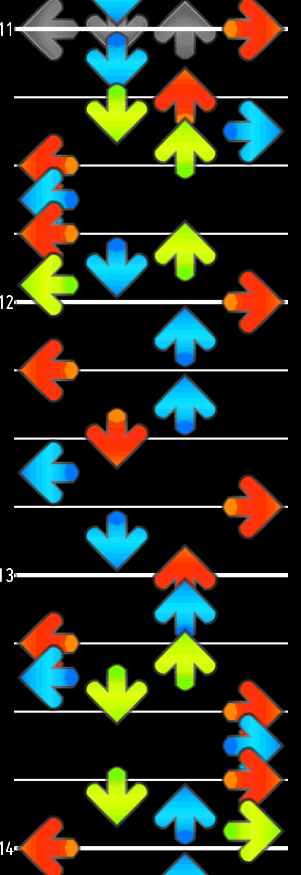
\includegraphics[width=0.16\textwidth]{boom-bombay-double-sideswitch-instead-of-jack.png}
		\\
		(a) Dr. Boom-Bombay \\
		(9, fort rapids vii)
	\end{tabular}
	\begin{tabular}{c}
		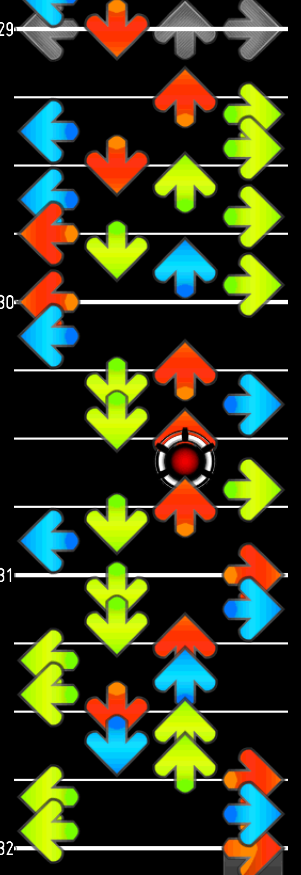
\includegraphics[width=0.16\textwidth]{toxic-xoverfs-avoid-doublestep.png}
		\\
		(b) Toxic \\
		(10/13, Sex'y Violation 2)
	\end{tabular}
	\end{center}
	\caption{Sometimes the algorithm was smarter than me.}
	\label{fig:surprise-sideswitch}
\end{figure}

{\bf Honourable Mentions.}
I omitted a table for the jackiest charts,
on account of most of them being either trivial beginner charts or extra-long megamixes.
One deserves a special mention:
Sandstorm (Jimmy Jawnz 2), shown in Figure~\ref{fig:hble-mention}(a),
has more than twice as many total jacks as the next jackiest chart,
clocking in at 1049 (78.5\%) with its 15 and 992 (69.6\%) with its 17.
And looking at that chart, can't you just hear Sandstorm playing in your head already?

I also wanted to highlight the chart with the most crossover switches,
shown in Figure~\ref{fig:hble-mention}(b),
mostly because the skittle notes should add some nice variety of colour to the paper
(with apologies to the dead-tree SIGBOVIK audience reading in greyscale).
Figure~\ref{fig:hble-mention}(c), with 2nd place in crossover switches following (b),
comes with an edit chart titled ``no sidefoots'',
and to be perfectly honest I just kept saying the word ``sidefoots'' to myself and giggling a lot while writing this paper.

\begin{figure*}[t]
	\begin{center}
	\begin{tabular}{c}
		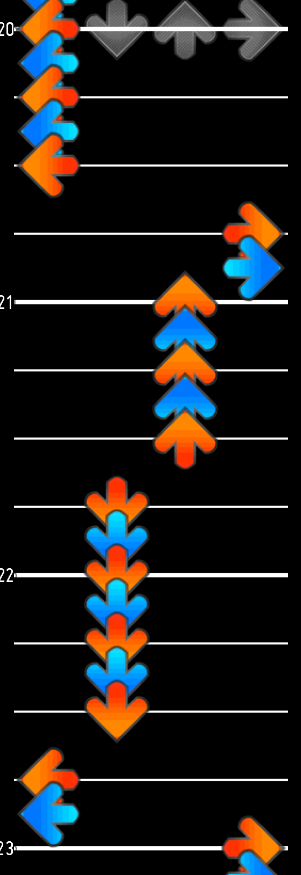
\includegraphics[width=0.16\textwidth]{sandstorm-jacks.png}
		\\
		(a) Sandstorm \\
		(15/17, J. Jawnz II)
	\end{tabular}
	\begin{tabular}{c}
		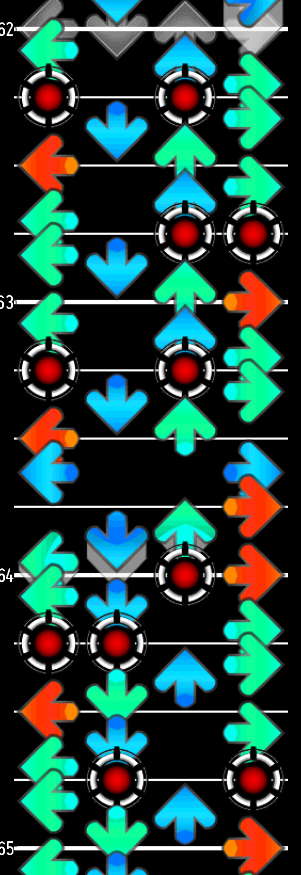
\includegraphics[width=0.16\textwidth]{heart-shooter-xover-fs.png}
		\\
		(b) Heart Shooter \\
		(11, VocaJawnz)
	\end{tabular}
	\begin{tabular}{c}
		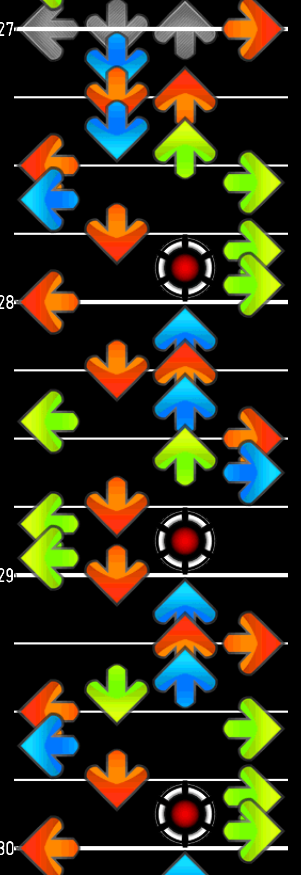
\includegraphics[width=0.16\textwidth]{slow-train-sidefoots.png}
		\\
		(c) '76 (Slow Train) \\
		(11, Mute Sims X)
	\end{tabular}
	\begin{tabular}{c}
		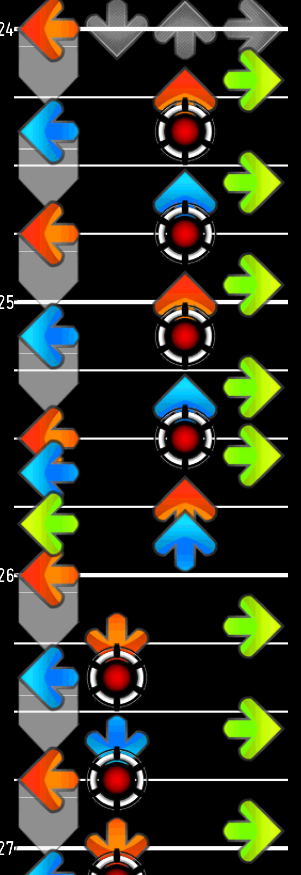
\includegraphics[width=0.16\textwidth]{conflict-cued-doublesteps.png}
		\\
		(d) Conflict \\
		(12, Stephcharts)
	\end{tabular}
	\begin{tabular}{c}
		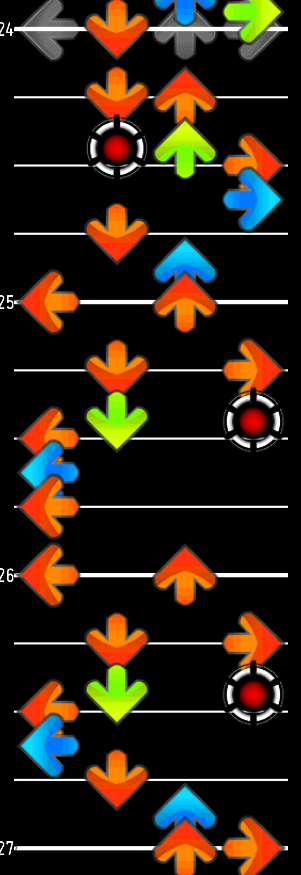
\includegraphics[width=0.16\textwidth]{matador-bracket-switch.png}
		\\
		(e) Matador \\
		(11, Valex 8)
	\end{tabular}
	\end{center}
	\caption{Miscellaneous interesting charts I discovered while browsing the giant spreadsheet.}
	\label{fig:hble-mention}
\end{figure*}

{\bf Sweet spot.}
Finally, in case it wasn't obvious in the tables, I'll point out that 9-15 is clearly the sweet spot of difficulties for technical stepcharts.

\section{Never Work}

Let's be honest: this isn't gonna be a paper trilogy.
Okay, with that said, here are some things that would be cool to implement in a fantasy universe with infinite free time.
(I have renamed this ``future'' work section accordingly.)

There are a few remaining cases the algorithm doesn't yet understand:
\begin{itemize}
	\item Doublesteps forced either by mine cues or by holds;
	\item Crossover and/or bracket jumps, not usually forced but often way less turny than the alternative;
	\item Forced footings across stream boundaries arising from bracket jumps or jump-footswitches.
\end{itemize}
For example, Figure~\ref{fig:hble-mention}(d) shows many sequential doublesteps, each forced by a mine cue,
but which the algorithm interprets as spins because the flipped stream length falls below \nflip.
Figure~\ref{fig:hble-mention}(e) shows an example of jump-footswitches
which the algorithm fails to count because it ignores the footing of jumps.

These patterns would all have to be identified heuristically.
Apart from that being more work than I wanted to do,
I also feel that adding too many heuristics to SIGBOVIK research
compromises the simple and innocent beauty of an implementation unbound by the demands of mainstream conferences.

\section{Conclusion}

Please accept my paper.
I worked hard on it.

%%%%%%%%%%%%%%%%%%%%%%%%%%%%%%%%%%%%%%%%%%%%%%%%%%%%%%%%%%%%%%%%%%%%%%%%%%%%%%%%

\bibliographystyle{abbrvnat}
\bibliography{citations}

\end{document}
